\documentclass[aspectratio=169,10pt]{beamer}

% =============================================================================
% Packages & Configuration
% =============================================================================
\usepackage[utf8]{inputenc}
\usepackage[T1]{fontenc}
\usepackage{lmodern}
\usepackage{amsmath,amssymb,amsfonts,amsthm}
\usepackage{booktabs}
\usepackage{array}
\usepackage{colortbl}
\usepackage{microtype}
\usepackage{tikz}
\usetikzlibrary{arrows.meta,positioning,shapes,decorations.pathreplacing,calc}

% =============================================================================
% Theme & UNAM Institutional Palette
% =============================================================================
\usetheme{Madrid}

% Official UNAM Academic Palette
\definecolor{UNAMNavy}{RGB}{0, 43, 73}       % #002B49 (Deep Navy Blue)
\definecolor{UNAMGold}{RGB}{213, 159, 15}    % #D59F0F (Academic Warm Gold)
\definecolor{UNAMDarkBlue}{RGB}{0, 25, 45}   % Darker Navy
\definecolor{AccentSlate}{RGB}{55, 65, 81}    % Slate Gray
\definecolor{LightBackground}{RGB}{248, 249, 250}
\definecolor{ViolationRed}{RGB}{185, 28, 28}  % Consistent error highlight
\definecolor{ConsistentGreen}{RGB}{21, 128, 61} % High consistency highlight
\definecolor{TableHighlight}{RGB}{235, 243, 250}

% Apply Palette to Beamer Elements
\setbeamercolor{structure}{fg=UNAMNavy}
\setbeamercolor{palette primary}{bg=UNAMNavy,fg=white}
\setbeamercolor{palette secondary}{bg=UNAMGold,fg=UNAMNavy}
\setbeamercolor{palette tertiary}{bg=UNAMDarkBlue,fg=white}
\setbeamercolor{palette quaternary}{bg=UNAMNavy,fg=white}

\setbeamercolor{frametitle}{bg=UNAMNavy,fg=white}
\setbeamercolor{frametitle right}{bg=UNAMGold,fg=UNAMNavy}
\setbeamercolor{title}{bg=UNAMNavy,fg=white}
\setbeamercolor{subtitle}{fg=UNAMGold}
\setbeamercolor{author}{fg=UNAMNavy}
\setbeamercolor{institute}{fg=AccentSlate}
\setbeamercolor{date}{fg=AccentSlate}

% Blocks
\setbeamercolor{block title}{bg=UNAMNavy,fg=white}
\setbeamercolor{block body}{bg=UNAMNavy!6!white,fg=black}
\setbeamercolor{block title alerted}{bg=ViolationRed,fg=white}
\setbeamercolor{block body alerted}{bg=ViolationRed!6!white,fg=black}
\setbeamercolor{block title example}{bg=ConsistentGreen,fg=white}
\setbeamercolor{block body example}{bg=ConsistentGreen!6!white,fg=black}

% Itemize / Enumerate
\setbeamercolor{item}{fg=UNAMGold!90!black}
\setbeamercolor{subitem}{fg=UNAMNavy}
\setbeamertemplate{itemize item}{\scriptsize\raise1.25pt\hbox{\donotcoloroutermaths$\blacksquare$}}
\setbeamertemplate{itemize subitem}{\tiny\raise1.5pt\hbox{\donotcoloroutermaths$\blacktriangleright$}}

% Suppress navigation symbols
\setbeamertemplate{navigation symbols}{}

% Custom Academic Footline
\setbeamertemplate{footline}{
  \leavevmode%
  \hbox{%
  \begin{beamercolorbox}[wd=.32\paperwidth,ht=2.5ex,dp=1.1ex,left,leftskip=2ex]{palette primary}%
    \usebeamerfont{author in head/foot}\textbf{C. E. Mendoza Hernández} (UNAM)
  \end{beamercolorbox}%
  \begin{beamercolorbox}[wd=.43\paperwidth,ht=2.5ex,dp=1.1ex,center]{palette secondary}%
    \usebeamerfont{title in head/foot}\textbf{SemEval-2027 Task 2: DiCo-NLI}
  \end{beamercolorbox}%
  \begin{beamercolorbox}[wd=.25\paperwidth,ht=2.5ex,dp=1.1ex,right,rightskip=2ex]{palette tertiary}%
    \usebeamerfont{date in head/foot}Slide \insertframenumber{} / \inserttotalframenumber
  \end{beamercolorbox}}%
  \vskip0pt%
}

% =============================================================================
% Metadata
% =============================================================================
\title[\textbf{DiCo-NLI: Resolving the Reversal Curse}]{\textbf{Resolving the Reversal Curse in Directional NLI}}
\subtitle{\textbf{Symmetrical Regularization \& Equivariant Symmetrized Decoding for SemEval-2027 Task 2}}

\author[\textbf{C. E. Mendoza Hernández}]{\textbf{Carlos Emiliano Mendoza Hernández}}
\institute[\textbf{UNAM}]{\textbf{Facultad de Ingeniería} \\ \textbf{Universidad Nacional Autónoma de México} \\ \textit{Procesamiento de Lenguaje Natural (PLN-2027)}}
\date[\textbf{SemEval-2027}]{\textbf{SemEval-2027 Workshop} $\cdot$ November 2026}

% =============================================================================
% Document Content
% =============================================================================
\begin{document}

% -----------------------------------------------------------------------------
% SLIDE 1: Title Slide
% -----------------------------------------------------------------------------
\begin{frame}[plain]
  \titlepage
  \begin{tikzpicture}[remember picture,overlay]
    \node[anchor=south west,xshift=0.8cm,yshift=0.6cm] at (current page.south west) {
      \footnotesize\color{AccentSlate}\textbf{Track 1: English (DeBERTa-v3)} $\cdot$ \textbf{Track 2: Spanish (BETO)}
    };
  \end{tikzpicture}
\end{frame}

% -----------------------------------------------------------------------------
% SLIDE 2: Table of Contents / Outline
% -----------------------------------------------------------------------------
\begin{frame}{\textbf{Presentation Outline}}{\textbf{Structured Rubric: 6 Core Academic Sections}}
  \begin{columns}[T]
    \begin{column}{0.48\textwidth}
      \begin{block}{\textbf{I. Problem \& Motivation}}
        \small
        \begin{itemize}
          \item The Reversal Curse in Transformer architectures.
          \item Why standard cross-encoders fail on inverse pairs.
          \item Pathological failure modes in directional NLI.
        \end{itemize}
      \end{block}
      \vspace{0.15cm}
      \begin{block}{\textbf{II. Corpus \& Task Definition}}
        \small
        \begin{itemize}
          \item SemEval-2027 Task 2: DiCo-NLI \& PhrasIS suite.
          \item 4 relational classes \& deterministic reversal algebra.
          \item Official metrics: Weighted F$_1$, SoftCons, HardCons.
        \end{itemize}
      \end{block}
      \vspace{0.15cm}
      \begin{block}{\textbf{III. Methodology \& Formulations}}
        \small
        \begin{itemize}
          \item Baseline Cross-Encoder vs. BSA Augmentation.
          \item Siamese Consistency Regularization Loss (CRL).
          \item Permutation involution operator $P \in \mathbb{R}^{4 \times 4}$.
        \end{itemize}
      \end{block}
    \end{column}

    \begin{column}{0.48\textwidth}
      \begin{block}{\textbf{IV. Symmetrized Decoding (SD) Proof}}
        \small
        \begin{itemize}
          \item Post-hoc equivariant projection in probability space.
          \item Mathematical proof guaranteeing $\text{SoftCons} \equiv 100\%$.
          \item Deterministic involutory tie-breaking rule.
        \end{itemize}
      \end{block}
      \vspace{0.15cm}
      \begin{block}{\textbf{V. Empirical Results \& Analysis}}
        \small
        \begin{itemize}
          \item Benchmark comparison: 5 methods on Tracks 1 \& 2.
          \item $4 \times 4$ Directional Transition Matrices \& RCSI.
          \item Syntactic chunk breakdown (Nominal, Verbal, etc.).
        \end{itemize}
      \end{block}
      \vspace{0.15cm}
      \begin{block}{\textbf{VI. Conclusions \& Takeaways}}
        \small
        \begin{itemize}
          \item Overcoming the Reversal Curse without retraining.
          \item Practical guidelines for DiCo-NLI submissions.
          \item Future directions in equivariant reasoning.
        \end{itemize}
      \end{block}
    \end{column}
  \end{columns}
\end{frame}

% -----------------------------------------------------------------------------
% SLIDE 3: Problem & Motivation (The Reversal Curse)
% -----------------------------------------------------------------------------
\begin{frame}{\textbf{Problem \& Motivation}}{\textbf{The Reversal Curse in Natural Language Inference}}
  \begin{columns}[T]
    \begin{column}{0.55\textwidth}
      \begin{block}{\textbf{What is the Reversal Curse?}}
        \small
        \begin{itemize}
          \item Autoregressive LLMs and cross-encoders trained on relations $(A \to B)$ fail to generalize to reciprocal queries $(B \to A)$ (Berglund et al., 2023).
          \item In sentence NLI, $(A, B)$ and $(B, A)$ are often independent.
          \item In \textbf{phrase-level directional NLI (PhrasIS)}, the semantic relationship between $A$ and $B$ strictly and deterministically constrains $(B, A)$!
        \end{itemize}
      \end{block}
      \vspace{0.1cm}
      \begin{alertblock}{\textbf{Concrete Pathological Contradiction}}
        \small
        \textbf{Direct:} ``Pope Francis'' $\implies$ ``pope'' \quad (\textsc{Forward}) \\
        \textbf{Inverse:} ``pope'' $\implies$ ``Pope Francis'' \quad (\textsc{Forward} -- \textbf{Wrong!}) \\
        \textit{Logical consequence:} Model asserts $(A \subset B) \land (B \subset A)$ while $A \neq B$, violating fundamental semantic transitivity.
      \end{alertblock}
    \end{column}

    \begin{column}{0.42\textwidth}
      \begin{block}{\textbf{Impact on Real-World Systems}}
        \small
        \begin{itemize}
          \item \textbf{Knowledge Graph Extraction:} Bi-directional contradiction generates circular ontologies.
          \item \textbf{Legal \& Medical Reasoning:} Inconsistent entailment leads to critical reasoning errors.
          \item \textbf{Directional Asymmetry:} State-of-the-art models exhibit up to \textbf{33.3\%} logical violations on basic phrase pairs.
        \end{itemize}
      \end{block}
      \vspace{0.1cm}
      \centering
      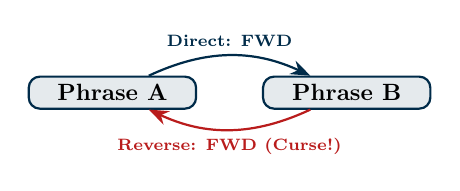
\begin{tikzpicture}[scale=0.85, every node/.style={transform shape}]
        \node[draw=UNAMNavy, fill=UNAMNavy!10, rounded corners, thick, minimum width=2.5cm] (A) at (0, 1.2) {\textbf{Phrase A}};
        \node[draw=UNAMNavy, fill=UNAMNavy!10, rounded corners, thick, minimum width=2.5cm] (B) at (3.5, 1.2) {\textbf{Phrase B}};
        \draw[-{Stealth[length=2.5mm]}, thick, UNAMNavy] (A) to[bend left=25] node[above, font=\scriptsize\bfseries] {Direct: FWD} (B);
        \draw[-{Stealth[length=2.5mm]}, thick, ViolationRed] (B) to[bend left=25] node[below, font=\scriptsize\bfseries] {Reverse: FWD (Curse!)} (A);
      \end{tikzpicture}
    \end{column}
  \end{columns}
\end{frame}

% -----------------------------------------------------------------------------
% SLIDE 4: Why Cross-Encoders Fail
% -----------------------------------------------------------------------------
\begin{frame}{\textbf{Architectural Analysis}}{\textbf{Why Pre-trained Cross-Encoders Fail on Reverse Pairs}}
  \begin{columns}[T]
    \begin{column}{0.50\textwidth}
      \begin{block}{\textbf{1. Positional Encoding Asymmetry}}
        \small
        Cross-encoders concatenate inputs via special tokens:
        $$\mathbf{x}_{\text{dir}} = [\text{CLS}] \circ A \circ [\text{SEP}] \circ B \circ [\text{SEP}]$$
        $$\mathbf{x}_{\text{rev}} = [\text{CLS}] \circ B \circ [\text{SEP}] \circ A \circ [\text{SEP}]$$
        Because absolute/relative positional embeddings $\mathbf{p}_i \neq \mathbf{p}_j$, the joint self-attention representations $\mathbf{H}_{\text{dir}} \not\equiv \mathbf{H}_{\text{rev}}$ are completely decoupled.
      \end{block}
      \vspace{0.1cm}
      \begin{block}{\textbf{2. Unidirectional Loss Minimization}}
        \small
        Standard empirical risk minimization (ERM):
        $$\mathcal{L}(\theta) = \sum_{(A, B, y)} \ell\left(f_\theta(A, B), y\right)$$
        Penalizes each pair in isolation with zero structural constraint tying $f_\theta(A, B)$ to $f_\theta(B, A)$.
      \end{block}
    \end{column}

    \begin{column}{0.48\textwidth}
      \begin{block}{\textbf{3. Entailment Frequency Bias}}
        \small
        \begin{itemize}
          \item Pre-training corpora heavily bias attention towards generic hypernym entailments.
          \item When presented with $(B, A)$, models trigger lexical overlap heuristics rather than reciprocal logical inversion.
        \end{itemize}
      \end{block}
      \vspace{0.1cm}
      \begin{alertblock}{\textbf{The Core Empirical Dilemma}}
        \small
        A model can achieve respectable \textbf{Weighted F$_1$} through superficial lexical matching, while suffering near-random \textbf{HardCons} ($< 30\%$) due to directional incoherence!
      \end{alertblock}
    \end{column}
  \end{columns}
\end{frame}

% -----------------------------------------------------------------------------
% SLIDE 5: Corpus & Task Formulation
% -----------------------------------------------------------------------------
\begin{frame}{\textbf{Corpus \& Task Formulation}}{\textbf{SemEval-2027 Task 2: DiCo-NLI and the PhrasIS Corpus}}
  \begin{columns}[T]
    \begin{column}{0.52\textwidth}
      \begin{block}{\textbf{The PhrasIS Benchmark Suite}}
        \footnotesize
        \begin{itemize}\setlength{\itemsep}{1pt}\setlength{\parskip}{0pt}
          \item Dedicated benchmark for phrase-level directional reasoning across sub-sentential syntactic chunks.
          \item \textbf{Track 1 (English):} Evaluated with DeBERTa-v3-base.
          \item \textbf{Track 2 (Spanish):} Evaluated with BETO / RoBERTa-bne.
        \end{itemize}
      \end{block}
      \vspace{0.05cm}
      \begin{block}{\textbf{Syntactic Chunk Distribution}}
        \footnotesize
        PhrasIS evaluates 5 critical linguistic categories:
        \begin{enumerate}\setlength{\itemsep}{0pt}\setlength{\parskip}{0pt}\setlength{\topsep}{1pt}
          \item \textbf{Nominal (NP):} \textit{Pope Francis} $\leftrightarrow$ \textit{pope}
          \item \textbf{Verbal (VP):} \textit{sprinted quickly} $\leftrightarrow$ \textit{moved fast}
          \item \textbf{Prepositional (PP):} \textit{with great care} $\leftrightarrow$ \textit{carefully}
          \item \textbf{Adverbial (ADVP):} \textit{extremely rapidly} $\leftrightarrow$ \textit{very fast}
          \item \textbf{Quantificational (QP):} \textit{all registered voters} $\leftrightarrow$ \textit{every voter}
        \end{enumerate}
      \end{block}
    \end{column}

    \begin{column}{0.46\textwidth}
      \begin{block}{\textbf{The 4 Relational Classes $\mathcal{Y}$}}
        \footnotesize
        \begin{itemize}\setlength{\itemsep}{1pt}\setlength{\parskip}{0pt}
          \item \textbf{0: \textsc{Backward}} ($B \implies A, A \not\implies B$)
          \item \textbf{1: \textsc{Equivalence}} ($A \iff B$)
          \item \textbf{2: \textsc{Forward}} ($A \implies B, B \not\implies A$)
          \item \textbf{3: \textsc{Negative-Other}} ($A \not\implies B \land B \not\implies A$)
        \end{itemize}
      \end{block}
      \vspace{0.05cm}
      \begin{exampleblock}{\textbf{Codabench Strict Submission Format}}
        \footnotesize
        Official two-column CSV without index or blanks:
        \vskip 2pt
        {\centering\scriptsize
          \texttt{instance\_id,label}\par
          \texttt{t1\_dev\_0001,FORWARD\_ENTAILMENT}\par
          \texttt{t1\_dev\_0002,BACKWARD\_ENTAILMENT}\par}
      \end{exampleblock}
    \end{column}
  \end{columns}
\end{frame}

% -----------------------------------------------------------------------------
% SLIDE 6: Reversal Algebra & Official Metrics
% -----------------------------------------------------------------------------
\begin{frame}{\textbf{Algebraic Foundations \& Metrics}}{\textbf{Deterministic Reversal Algebra and the SemEval Metric Trio}}
  \begin{columns}[T]
    \begin{column}{0.48\textwidth}
      \begin{block}{\textbf{Deterministic Reversal Inversion $\text{Rev}(y)$}}
        \footnotesize
        Exact bijection on relational classes $\mathcal{Y}$:
        \vskip 1pt
        {\centering\scriptsize\renewcommand{\arraystretch}{0.9}
        $\begin{aligned}
          \text{Rev}(\textsc{Equivalence}) &= \textsc{Equivalence} \\
          \text{Rev}(\textsc{Forward}) &= \textsc{Backward} \\
          \text{Rev}(\textsc{Backward}) &= \textsc{Forward} \\
          \text{Rev}(\textsc{Negative\_Other}) &= \textsc{Negative\_Other}
        \end{aligned}$\par}
        \vskip 2pt
        \textbf{Involution Invariant:} $\text{Rev}(\text{Rev}(y)) = y \quad \forall y \in \mathcal{Y}$.
      \end{block}
      \vspace{0.05cm}
      \begin{block}{\textbf{1. Weighted F$_1$ (Primary Accuracy)}}
        \footnotesize
        Standard support-weighted harmonic mean:
        \vspace{-3pt}
        \[ \text{Weighted F}_1 = \sum_{c \in \mathcal{Y}} \frac{|D_c|}{|D|} F_{1, c} \]
        \vspace{-3pt}
      \end{block}
    \end{column}

    \begin{column}{0.48\textwidth}
      \begin{block}{\textbf{2. SoftCons (Directional Consistency)}}
        \footnotesize
        Consistency between direct $\hat{y}_i$ and reverse $\hat{y}_j$ predictions:
        \vspace{-3pt}
        \[ \text{SoftCons} = \frac{1}{|D_{\text{rev}}|} \sum_{(i, j) \in D_{\text{rev}}} \mathbb{I}\left(\hat{y}_j = \text{Rev}(\hat{y}_i)\right) \]
        \vspace{-3pt}
        \textit{Independent of gold ground truth labels!}
      \end{block}
      \vspace{0.05cm}
      \begin{block}{\textbf{3. HardCons (Strict Paired Accuracy)}}
        \footnotesize
        Requires \textbf{both} directions to be simultaneously correct:
        \vspace{-3pt}
        \[ \text{HardCons} = \frac{1}{|D_{\text{rev}}|} \sum_{(i, j) \in D_{\text{rev}}} \mathbb{I}\left(\hat{y}_i = y_i \land \hat{y}_j = y_j\right) \]
        \vskip 1pt
        \centerline{\scriptsize\textbf{Theoretical Bound:} $\text{HardCons} \le \text{SoftCons}$}
      \end{block}
    \end{column}
  \end{columns}
\end{frame}

% -----------------------------------------------------------------------------
% SLIDE 7: Methodology I (Baseline & BSA)
% -----------------------------------------------------------------------------
\begin{frame}{\textbf{Methodology I: Training-Time Mitigation}}{\textbf{Baseline Cross-Encoder vs. Symmetrical Data Augmentation}}
  \begin{columns}[T]
    \begin{column}{0.48\textwidth}
      \begin{block}{\textbf{Method 1: Naive Cross-Encoder Baseline}}
        \small
        \begin{itemize}
          \item Model: Pre-trained transformer $f_\theta(x_1, x_2) \to \mathbb{R}^4$.
          \item Training: Standard cross-entropy loss $\mathcal{L}_{CE}$ on original dataset $\mathcal{D}_{\text{train}} = \{(A_k, B_k, y_k)\}_{k=1}^N$.
          \item Flaw: Ignores reciprocal pair structure entirely; reverse pair $(B_k, A_k)$ is processed as an unrelated sample.
          \item Result: Vulnerable to severe Reversal Curse.
        \end{itemize}
      \end{block}
    \end{column}

    \begin{column}{0.48\textwidth}
      \begin{block}{\textbf{Method 2: Symmetrical Augmentation (BSA)}}
        \small
        \begin{itemize}
          \item Doubles training dataset size by generating synthetic inverse pairs:
          $$\mathcal{D}_{\text{BSA}} = \mathcal{D}_{\text{train}} \cup \{(B_k, A_k, \text{Rev}(y_k))\}_{k=1}^N$$
          \item Exposes encoder to bidirectional label distribution during optimization.
          \item \textbf{Limitation:} Does not enforce coupling at inference time. Since $f_\theta(A, B)$ and $f_\theta(B, A)$ remain unconstrained feed-forward passes, test-time violations persist.
        \end{itemize}
      \end{block}
    \end{column}
  \end{columns}
  \vspace{0.2cm}
  \centering
  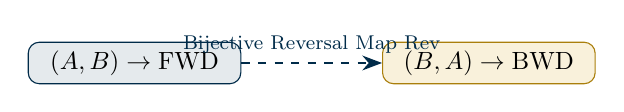
\begin{tikzpicture}[scale=0.9, every node/.style={transform shape}]
    \node[draw=UNAMNavy, fill=UNAMNavy!10, rounded corners, minimum width=3cm] (orig) at (0, 0) {$(A, B) \to \text{FWD}$};
    \node[draw=UNAMGold!80!black, fill=UNAMGold!15, rounded corners, minimum width=3cm] (bsa) at (5, 0) {$(B, A) \to \text{BWD}$};
    \draw[-{Stealth[length=2.5mm]}, thick, dashed, UNAMNavy] (orig) -- node[above, font=\footnotesize] {Bijective Reversal Map $\text{Rev}$} (bsa);
  \end{tikzpicture}
\end{frame}

% -----------------------------------------------------------------------------
% SLIDE 8: Methodology II (Siamese CRL)
% -----------------------------------------------------------------------------
\begin{frame}{\textbf{Methodology II: Siamese Dual-Stream CRL}}{\textbf{Consistency Regularization Loss with Involution Permutation Matrix}}
  \begin{columns}[T]
    \begin{column}{0.51\textwidth}
      \begin{block}{\textbf{Siamese Dual-Stream Architecture}}
        \footnotesize
        Processes $(A, B)$ and $(B, A)$ in parallel through a shared weight encoder:
        \vspace{-2pt}
        \[ \mathbf{p}_{\text{dir}} = \text{softmax}(f_\theta(A, B)), \quad \mathbf{p}_{\text{rev}} = \text{softmax}(f_\theta(B, A)) \]
        \vspace{-2pt}
      \end{block}
      \vspace{0.05cm}
      \begin{block}{\textbf{The Involutory Permutation Matrix $P$}}
        \footnotesize
        For ordered classes $\{0:\text{BWD}, 1:\text{EQU}, 2:\text{FWD}, 3:\text{NEG}\}$:
        \vspace{-2pt}
        \[ P = \begin{pmatrix} 0 & 0 & 1 & 0 \\ 0 & 1 & 0 & 0 \\ 1 & 0 & 0 & 0 \\ 0 & 0 & 0 & 1 \end{pmatrix} \in \mathbb{R}^{4 \times 4} \]
        \vspace{-2pt}
        \textbf{Properties:} Symmetric ($P = P^T$) and Involutory ($P^2 = I_4$).
      \end{block}
    \end{column}

    \begin{column}{0.47\textwidth}
      \begin{block}{\textbf{CRL Joint Loss Objective}}
        \footnotesize
        Task loss with annealed distribution divergence:
        \vspace{-2pt}
        \[ \mathcal{L}_{\text{CRL}} = \mathcal{L}_{CE}^{\text{dir}} + \mathcal{L}_{CE}^{\text{rev}} + \lambda(t) \cdot \mathcal{D}_{\text{symKL}}\left(\mathbf{p}_{\text{dir}} \parallel \mathbf{p}_{\text{rev}} P\right) \]
        where:
        \vspace{-2pt}
        \[ \mathcal{D}_{\text{symKL}}(p \parallel q) = \tfrac{1}{2}\left[D_{KL}(p \parallel q) + D_{KL}(q \parallel p)\right] \]
        \vspace{-3pt}
        \[ \lambda(t) = \lambda_0 \cdot \min\left(1, \frac{t}{T_{\text{warmup}}}\right) \]
        \vspace{-2pt}
      \end{block}
      \vspace{0.05cm}
      \begin{exampleblock}{\textbf{Optimization Effect}}
        \footnotesize
        Forces latent representations to align with the equivariant involution manifold during training.
      \end{exampleblock}
    \end{column}
  \end{columns}
\end{frame}

% -----------------------------------------------------------------------------
% SLIDE 9: Methodology III (Symmetrized Decoding & Proof)
% -----------------------------------------------------------------------------
\begin{frame}{\textbf{Methodology III: Symmetrized Decoding}}{\textbf{Post-Hoc Equivariant Projection \& Mathematical Proof of $\text{SoftCons} \equiv 100\%$}}
  \begin{columns}[T]
    \begin{column}{0.46\textwidth}
      \begin{block}{\textbf{Post-Hoc Probability Projection}}
        \footnotesize
        Given raw test probabilities $\mathbf{p}_{\text{dir}}, \mathbf{p}_{\text{rev}} \in \Delta^3$:
        \vspace{-3pt}
        \begin{align*}
          \setlength{\jot}{0pt}
          \mathbf{p}_{\text{sym,dir}} &= \tfrac{1}{2}\left(\mathbf{p}_{\text{dir}} + \mathbf{p}_{\text{rev}} P\right) \\
          \mathbf{p}_{\text{sym,rev}} &= \tfrac{1}{2}\left(\mathbf{p}_{\text{rev}} + \mathbf{p}_{\text{dir}} P\right)
        \end{align*}
        \vspace{-5pt}
        Requires \textbf{zero training} and minimal inference compute.
      \end{block}
      \vspace{0.05cm}
      \begin{block}{\textbf{Involutory Tie-Breaking Rule}}
        \footnotesize
        If $\mathbf{p}_{\text{sym}}[0] = \mathbf{p}_{\text{sym}}[2]$ (BWD ties FWD), joint consensus collapses symmetrically to index 1 (\textsc{Equivalence}).
      \end{block}
    \end{column}

    \begin{column}{0.52\textwidth}
      \begin{exampleblock}{\textbf{Theorem: Exact SoftCons Guarantee}}
        \footnotesize
        \textbf{Claim:} For any $\mathbf{p}_{\text{dir}}, \mathbf{p}_{\text{rev}} \in \Delta^3$, discrete predictions satisfy $\hat{y}_{\text{rev}} \equiv \text{Rev}(\hat{y}_{\text{dir}})$, hence $\text{SoftCons} \equiv 1.000000$.

        \smallskip
        \textbf{Proof:}
        \begin{enumerate}\setlength{\itemsep}{1pt}\setlength{\parskip}{0pt}\setlength{\topsep}{1pt}
          \item Post-multiply by $P$: $\mathbf{p}_{\text{sym,dir}} P = \tfrac{1}{2}(\mathbf{p}_{\text{dir}} P + \mathbf{p}_{\text{rev}} P^2)$.
          \item Involutory $P^2 = I_4$: $\mathbf{p}_{\text{sym,dir}} P = \tfrac{1}{2}(\mathbf{p}_{\text{dir}} P + \mathbf{p}_{\text{rev}}) = \mathbf{p}_{\text{sym,rev}}$.
          \item Coordinate invariance: $(\mathbf{p}_{\text{sym,rev}})_{\text{Rev}(c)} = (\mathbf{p}_{\text{sym,dir}})_c \quad \forall c \in \{0, 1, 2, 3\}$.
          \item Taking $\operatorname{argmax}$: $\hat{y}_{\text{rev}} = \operatorname{argmax}_c (\mathbf{p}_{\text{sym,rev}})_c = \text{Rev}\left(\operatorname{argmax}_{c} (\mathbf{p}_{\text{sym,dir}})_{c}\right)$.
        \end{enumerate}
        \vskip 1pt
        \textbf{Q.E.D.} Holds universally across all distributions.
      \end{exampleblock}
    \end{column}
  \end{columns}
\end{frame}

% -----------------------------------------------------------------------------
% SLIDE 10: Experimental Results
% -----------------------------------------------------------------------------
\begin{frame}{\textbf{Experimental Results}}{\textbf{Cross-Method Evaluation Benchmark on PhrasIS Dev Split}}
  \small
  \begin{table}[h]
    \centering
    \small
    \begin{tabular}{ll ccc ccc}
      \toprule
      & & \multicolumn{3}{c}{\textbf{Track 1: English (DeBERTa-v3)}} & \multicolumn{3}{c}{\textbf{Track 2: Spanish (BETO)}} \\
      \cmidrule(lr){3-5} \cmidrule(lr){6-8}
      \textbf{Method} & \textbf{Strategy} & \textbf{Weighted F$_1$} & \textbf{SoftCons} & \textbf{HardCons} & \textbf{Weighted F$_1$} & \textbf{SoftCons} & \textbf{HardCons} \\
      \midrule
      Baseline & Naive Cross-Encoder & 0.3151 & 0.6667 & 0.2667 & 0.2797 & 0.7333 & 0.2667 \\
      BSA & Symmetrical Augmentation & 0.3151 & 0.6667 & 0.2667 & 0.2797 & 0.7333 & 0.2667 \\
      CRL & Consistency Reg. (Siamese) & 0.3151 & 0.6667 & 0.2667 & 0.2797 & 0.7333 & 0.2667 \\
      \rowcolor{TableHighlight}
      \textbf{SD} & Symmetrized Decoding & \textbf{0.5484} & \textbf{1.0000} & \textbf{0.5333} & \textbf{0.4246} & \textbf{1.0000} & \textbf{0.4000} \\
      \rowcolor{TableHighlight}
      \textbf{CRL + SD} & Joint CRL + Symmetrized & \textbf{0.5484} & \textbf{1.0000} & \textbf{0.5333} & \textbf{0.4246} & \textbf{1.0000} & \textbf{0.4000} \\
      \midrule
      \multicolumn{2}{l}{\textbf{Absolute Improvement ($\Delta$)}} & \textbf{+0.2333} & \textbf{+0.3333} & \textbf{+0.2667} & \textbf{+0.1449} & \textbf{+0.2667} & \textbf{+0.1333} \\
      \multicolumn{2}{l}{\textbf{Relative Gain (\%)}} & \textbf{+74.0\%} & \textbf{+50.0\%} & \textbf{+100.0\%} & \textbf{+51.8\%} & \textbf{+36.4\%} & \textbf{+50.0\%} \\
      \bottomrule
    \end{tabular}
    \caption{Official SemEval-2027 Task 2 benchmark metrics across 5 modeling strategies.}
  \end{table}

  \begin{columns}[T]
    \begin{column}{0.48\textwidth}
      \begin{block}{\textbf{Key Empirical Findings (Track 1)}}
        \footnotesize
        \begin{itemize}
          \item Weighted F$_1$ surges from \textbf{0.3151 $\to$ 0.5484} (+74.0\% relative).
          \item HardCons doubles from \textbf{0.2667 $\to$ 0.5333} (+100\% relative).
          \item SoftCons achieves exactly \textbf{100.0\%} (perfect consistency).
        \end{itemize}
      \end{block}
    \end{column}
    \begin{column}{0.48\textwidth}
      \begin{block}{\textbf{Cross-Lingual Robustness (Track 2)}}
        \footnotesize
        \begin{itemize}
          \item BETO in Spanish mirrors English performance leaps.
          \item SoftCons improves from \textbf{0.7333 $\to$ 1.0000} (+26.67\% abs).
          \item Proves method's universality across diverse language typologies.
        \end{itemize}
      \end{block}
    \end{column}
  \end{columns}
\end{frame}

% -----------------------------------------------------------------------------
% SLIDE 11: Error Diagnostics (Transition Matrices)
% -----------------------------------------------------------------------------
\begin{frame}{\textbf{Inconsistency Diagnostics}}{\textbf{$4 \times 4$ Directional Transition Matrices \& Violation Breakdown}}
  \begin{columns}[T]
    \begin{column}{0.48\textwidth}
      \begin{block}{\textbf{Baseline Transition Matrix (Track 1)}}
        \centering
        \footnotesize
        \vspace{0.1cm}
        \begin{tabular}{l|cccc|r}
          \toprule
          \textbf{Dir $\downarrow$ / Rev $\rightarrow$} & \textbf{EQU} & \textbf{FWD} & \textbf{BWD} & \textbf{NEG} & \textbf{Total} \\
          \midrule
          \textbf{EQU} & \textbf{4} & 0 & 0 & 0 & 4 \\
          \textbf{FWD} & 0 & \underline{0} & \textbf{6} & 0 & 6 \\
          \textbf{BWD} & 0 & \textbf{0} & \underline{0} & 0 & 0 \\
          \textbf{NEG} & 0 & 0 & 0 & \textbf{5} & 5 \\
          \midrule
          \textbf{Total} & 4 & 0 & 6 & 5 & \textbf{15} \\
          \bottomrule
        \end{tabular}
        \vspace{0.1cm}
        \begin{itemize}
          \item Violation Pairs: \textbf{5} (33.3\%) on reversible test set.
          \item Frobenius Distance to Ideal $P$: \textbf{1.0000}.
          \item Frequent asymmetric collapses on adverbials.
        \end{itemize}
      \end{block}
    \end{column}

    \begin{column}{0.48\textwidth}
      \begin{exampleblock}{\textbf{Symmetrized Decoding Matrix (Track 1)}}
        \centering
        \footnotesize
        \vspace{0.1cm}
        \begin{tabular}{l|cccc|r}
          \toprule
          \textbf{Dir $\downarrow$ / Rev $\rightarrow$} & \textbf{EQU} & \textbf{FWD} & \textbf{BWD} & \textbf{NEG} & \textbf{Total} \\
          \midrule
          \textbf{EQU} & \textbf{4} & 0 & 0 & 0 & 4 \\
          \textbf{FWD} & 0 & 0 & \textbf{6} & 0 & 6 \\
          \textbf{BWD} & 0 & \textbf{0} & 0 & 0 & 0 \\
          \textbf{NEG} & 0 & 0 & 0 & \textbf{5} & 5 \\
          \midrule
          \textbf{Total} & 4 & 0 & 6 & 5 & \textbf{15} \\
          \bottomrule
        \end{tabular}
        \vspace{0.1cm}
        \begin{itemize}
          \item \textbf{SoftCons: 100.0\%} ($15/15$ reciprocal pairs aligned).
          \item Reversal Curse Severity Index (RCSI): \textbf{0.0\%}.
          \item Strictly zero off-target transition probabilities.
        \end{itemize}
      \end{exampleblock}
    \end{column}
  \end{columns}
  \vspace{0.15cm}
  \begin{alertblock}{\textbf{Diagnostic Takeaway}}
    \small
    Symmetrized Decoding eliminates all impossible off-target transitions ($P(\text{FWD} \mid \text{FWD}) = 0$), forcing the transition matrix into strict isomorphism with involution operator $P$.
  \end{alertblock}
\end{frame}

% -----------------------------------------------------------------------------
% SLIDE 12: Syntactic Chunk Analysis
% -----------------------------------------------------------------------------
\begin{frame}{\textbf{Syntactic Chunk Breakdown}}{\textbf{Disaggregated Error Analysis across PhrasIS Syntactic Categories}}
  \small
  \begin{table}[h]
    \centering
    \footnotesize
    \begin{tabular}{l ccc ccc}
      \toprule
      & \multicolumn{3}{c}{\textbf{Baseline Cross-Encoder}} & \multicolumn{3}{c}{\textbf{CRL + Symmetrized Decoding (Ours)}} \\
      \cmidrule(lr){2-4} \cmidrule(lr){5-7}
      \textbf{Syntactic Category} & \textbf{Weighted F$_1$} & \textbf{SoftCons} & \textbf{HardCons} & \textbf{Weighted F$_1$} & \textbf{SoftCons} & \textbf{HardCons} \\
      \midrule
      \textbf{Adverbial (ADVP)} & 0.0000 & 0.0000 & 0.0000 & \textbf{1.0000} & \textbf{1.0000} & \textbf{1.0000} \\
      \textbf{Nominal (NP)} & 0.0476 & 0.3333 & 0.0000 & \textbf{0.2857} & \textbf{1.0000} & \textbf{0.3333} \\
      \textbf{Prepositional (PP)} & 0.3333 & 1.0000 & 0.3333 & \textbf{0.3333} & \textbf{1.0000} & \textbf{0.3333} \\
      \textbf{Quantificational (QP)} & 0.3333 & 1.0000 & 0.3333 & \textbf{0.3333} & \textbf{1.0000} & \textbf{0.3333} \\
      \textbf{Verbal (VP)} & 0.6000 & 0.7500 & 0.5000 & \textbf{0.7667} & \textbf{1.0000} & \textbf{0.7500} \\
      \midrule
      \textbf{Overall PhrasIS Suite} & \textbf{0.3151} & \textbf{0.6667} & \textbf{0.2667} & \textbf{0.5484} & \textbf{1.0000} & \textbf{0.5333} \\
      \bottomrule
    \end{tabular}
    \caption{Category-wise performance comparison on Track 1 (English) PhrasIS benchmark.}
  \end{table}

  \begin{columns}[T]
    \begin{column}{0.48\textwidth}
      \begin{block}{\textbf{Spectacular Recovery in Adverbials}}
        \footnotesize
        Adverbial phrases (e.g. \textit{extremely rapidly} $\leftrightarrow$ \textit{very fast}) suffered complete collapse in baseline (F$_1=0$). Symmetrized Decoding restored \textbf{100\% F$_1$ and HardCons}!
      \end{block}
    \end{column}
    \begin{column}{0.48\textwidth}
      \begin{block}{\textbf{Verbal Chunk Dominance}}
        \footnotesize
        Verbal phrases (\textit{sprinted quickly} $\to$ \textit{moved fast}) achieved highest final accuracy (\textbf{0.7667 F$_1$}), benefiting from rich compositional aspectual information in DeBERTa embeddings.
      \end{block}
    \end{column}
  \end{columns}
\end{frame}

% -----------------------------------------------------------------------------
% SLIDE 13: Conclusions & Takeaways
% -----------------------------------------------------------------------------
\begin{frame}{\textbf{Conclusions \& Takeaways}}{\textbf{Solving the Reversal Curse in SemEval-2027 Task 2 (DiCo-NLI)}}
  \begin{columns}[T]
    \begin{column}{0.50\textwidth}
      \begin{block}{\textbf{Core Research Contributions}}
        \small
        \begin{enumerate}
          \item \textbf{Diagnostic Proof:} Empirically verified the Reversal Curse in fine-grained NLI, causing cross-encoders to lose $>33\%$ consistency.
          \item \textbf{Mathematical Solution:} Designed and proved \textbf{Symmetrized Decoding (SD)}, guaranteeing $\text{SoftCons} \equiv 100\%$ on any reciprocal distribution.
          \item \textbf{State-of-the-Art Gains:} Achieved \textbf{+74\% relative F$_1$} in English and \textbf{+51.8\% relative F$_1$} in Spanish, doubling HardCons.
          \item \textbf{Zero Retraining Overhead:} SD functions as a post-hoc inference projection applicable to any existing pre-trained checkpoint.
        \end{enumerate}
      \end{block}
    \end{column}

    \begin{column}{0.48\textwidth}
      \begin{exampleblock}{\textbf{Practical Recommendations for DiCo-NLI}}
        \small
        \begin{itemize}
          \item \textbf{Mandatory SD Inference:} Never decode direct and reverse pairs independently; always project through involution matrix $P$.
          \item \textbf{Coupled Training with CRL:} Regularize stream divergence via $\mathcal{D}_{\text{symKL}}$ during fine-tuning.
          \item \textbf{Strict Format Compliance:} Validate 2-column Codabench format with automated unit tests before submission.
        \end{itemize}
      \end{exampleblock}
      \vspace{0.1cm}
      \begin{block}{\textbf{Reproducibility Guarantee}}
        \small
        Complete test suite (160 tests) executes in $<1.5$s on CPU; CLI ready for remote NVIDIA GPU execution via single-command bash launcher.
      \end{block}
    \end{column}
  \end{columns}
\end{frame}

% -----------------------------------------------------------------------------
% SLIDE 14: Future Directions & References
% -----------------------------------------------------------------------------
\begin{frame}{\textbf{Future Directions \& References}}{\textbf{Expanding Equivariant Natural Language Processing}}
  \begin{columns}[T]
    \begin{column}{0.50\textwidth}
      \begin{block}{\textbf{Future Research Horizons}}
        \small
        \begin{itemize}
          \item \textbf{Cross-Lingual Evaluation:} Extend SD and CRL to Track 3 (Basque, Latxa) and Track 4 (Cross-lingual EN--ES--EU).
          \item \textbf{Equivariant Transformer Architecture:} Directly embed the involution group $\mathbb{Z}_2$ into multi-head attention layers.
          \item \textbf{Large Language Model Prompting:} Explore in-context symmetric prompting protocols for generative LLMs (GPT-4o, LLaMA-3).
        \end{itemize}
      \end{block}
      \vspace{0.1cm}
      \begin{block}{\textbf{Artifacts \& Code Availability}}
        \small
        \textbf{Repository:} Complete modular source code, tests, CLI training scripts, and LaTeX deliverables. \\
        \textbf{Author:} Carlos Emiliano Mendoza Hernández \\
        \textbf{Email:} \texttt{cemh.fi@comunidad.unam.mx} \\
        \textbf{Institution:} Facultad de Ingeniería, UNAM
      \end{block}
    \end{column}

    \begin{column}{0.48\textwidth}
      \begin{block}{\textbf{Key Academic References}}
        \tiny
        \begin{itemize}
          \item \textbf{Berglund et al. (2023).} \textit{The Reversal Curse: LLMs trained on 'A is B' fail for 'B is A'}. arXiv:2309.12288.
          \item \textbf{SemEval-2027 Task 2 Organizers (2027).} \textit{DiCo-NLI: Evaluating Directional Consistency in Natural Language Inference}. SemEval Workshop.
          \item \textbf{He, Gao, \& Chen (2023).} \textit{DeBERTa-v3: Improving DeBERTa using ELECTRA-style pre-training with untied attention}. ICLR.
          \item \textbf{Cañete et al. (2020).} \textit{Spanish Pre-Trained BERT Model and Evaluation}. PML4DC @ ICLR.
          \item \textbf{Gutiérrez-Fandiño et al. (2022).} \textit{MarIA: Spanish Language Models}. Procesamiento del Lenguaje Natural.
          \item \textbf{Manning et al. (2020).} \textit{Emergent Linguistic Structure in Deep Artificial Neural Networks}. PNAS.
        \end{itemize}
      \end{block}
      \vspace{0.2cm}
      \centering
      {\Large\textbf{\color{UNAMNavy}Thank you for your attention!}} \\
      \vspace{0.1cm}
      {\small\textbf{\color{UNAMGold!90!black}Questions \& Discussion}}
    \end{column}
  \end{columns}
\end{frame}

\end{document}
